\documentclass[a4paper]{article}
\usepackage{tikz}
\usepackage{multicol}
\usepackage{longtable}
\usepackage{url}
\usepackage{hyperref}
\newtheorem{theorem}{Theorem}

\title{A Decomposition Model for the NoWaitHFS Problem}
\author{Ahmed Missaoui and Helmut Simonis} 
\begin{document}
\maketitle
\begin{abstract}
\end{abstract}

\section{Model}
We describe a decomposition model for a NoWaitHFS problem with $n$ jobs $J$ and $s$ stages $S$, scheduled on a set of disjunctive machines $M$.
Each job consists of $s$ tasks with start time $s_{ij}$ and duration $d_{ij}$ for stage $i$ of job $j$, assigned to machine $m_{ij}$. 
Each stage has the same number of machines $m_{s}$.

We define the schedule by giving an assigned machine $m_{ij}$ for each task, these values range from 1 to $m_{s}$. 
We also define the position $p_{ij}$ of a task on its assigned machine, these values range from 1 to a maximum of $n$. Two tasks of the same stage $i$ only 
can have the same values $p_{ij}$ if they are scheduled on different machines.

Therefore the following invariant must hold:
\begin{equation}
\forall_{j_{1},j_{2} \in J\ s.t.\ j_{1} \neq j_{2}}\forall_{i \in S}:\quad (m_{ij_{1}} \neq m_{ij_{2}} \vee p_{ij_{1}} \neq p_{ij_{2}})
\end{equation}

The positions of two jobs in two consecutive stages must be compatible
\begin{equation}
\forall_{j_{1},j_{2} \in J\ s.t.\ j_{1} \neq j_{2}}\forall_{1 \leq i < s}:\quad (m_{ij_{1}} = m_{ij_{2}} \land p_{i_{1}} < p_{ij_{2}}) \Rightarrow (m_{i+1,j_{1}} \neq m_{i+1,j_{2}} \vee p_{i+1,j_{1}} < p_{i+1,j_{2}}) \label{eq:order}
\end{equation}
If two jobs $j_{1}$ and $j_{2}$ are assigned on the same machine in stage $i$, then they must be either assigned to different machines in stage $i+1$, or they must 
be in the same order in both stages. The start time $s_{i+1,j_{2}}=s_{ij_{2}}+d_{ij_{2}}$ of task $j_{2}$ in stage $i+1$ can never be before 
the start $s_{i+1,j_{1}}=s_{ij_{1}} + d_{ij_{1}}$ of the task for job $j_{1}$ in that stage, as $s_{ij_{2}}$ is already greater than or equal to $s_{ij_{1}}+d_{ij_{1}}$, since $j_{2}$ follows $j_{1}$ in stage $i$.
  


The start times within a job are linked by equality constraints, as soon as one stage finished, the next stage must start, there is no wait between the tasks of the same job.

\begin{equation}
\forall_{j \in J}\forall_{1\leq i<s}:\quad s_{i+1,j} = s_{ij}+d_{ij} \label{eq:temp1}
\end{equation}

The total completion time $C_{\max}$ of the schedule is defined as
\begin{equation}
C_{\max} = \max_{j \in J} s_{sj}+d_{sj} \label{eq:temp2}
\end{equation}
The overall end of the schedule is the last of the ends of any job. The objective is to minimize the overall completion time.

The following constraint links the ordering on the machines with the start times. If two jobs $j_{1}$ and $j_{2}$ in stage $i$ are scheduled on the same machine, then their start times must be follow the ordering of the jobs on the machine:

\begin{equation}
\forall_{j_{1},j_{2} \in J\ s.t.\ j_{1} \neq j_{2}}\forall_{i \in S}:\quad m_{ij_{1}} = m_{ij_{2}} \land p_{ij_{1}} < p_{ij_{2}} \Rightarrow s_{ij_{2}} \geq s_{ij_{1}} + d_{ij_{1}} \label{eq:temp3}
\end{equation}

Note that once the ordering of the jobs on the machine is given, the best resulting schedule can be obtained by solving the set of constraints~(\ref{eq:temp1}) to~(\ref{eq:temp3}) without search.

\subsection{Reversing Job Order}

We have stated in constraint~(\ref{eq:order}) that if one job follows another in some stage $i$, it must also follow that job in the next stage, unless it is assigned to another machine. 
The example in Figure~\ref{fig:order2} shows that this is not necessarily true for later stages. We consider two jobs $j_{1}$ and $j_{2}$, which on the first and third stage are running 
on the same machine $m_{11}$ and $m_{31}$, respectively. In stage two they run on different machines $m_{21}$ and $m_{22}$. While $j_{1}$ is before $j_{2}$ in stage 1, $j_{2}$ is before $j_{1}$ on stage 3, the order is reversed.
\begin{figure}[htbp]
\caption{\label{fig:order2} Order Inversion Example (Job View, Colored by Stage)}
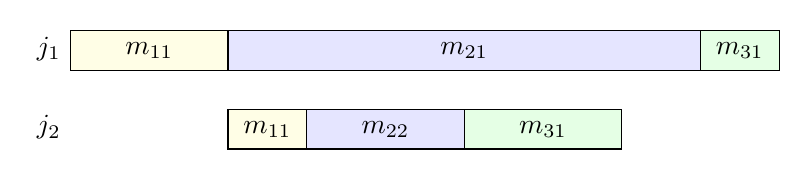
\begin{tikzpicture}
\node[above left] (j1) at (0,2) {$j_{1}$};

\draw[draw=black,fill=yellow!10] (0,2) rectangle node {$m_{11}$} (2,2.5);
\draw[draw=black,fill=blue!10] (2,2) rectangle node {$m_{21}$} (8,2.5);
\draw[draw=black,fill=green!10] (8,2) rectangle node {$m_{31}$} (9,2.5);

\node[above left] (j2) at (0,1) {$j_{2}$};

\draw[draw=black,fill=yellow!10] (2,1) rectangle node {$m_{11}$} (3,1.5);
\draw[draw=black,fill=blue!10] (3,1) rectangle node {$m_{22}$} (5,1.5);
\draw[draw=black,fill=green!10] (5,1) rectangle node {$m_{31}$} (7,1.5);

\end{tikzpicture}
\end{figure}

But a job can only overtake another if the duration of the tasks in the stages are widely different. The following is a necessary condition
\begin{equation}
d_{2j_{1}} \geq d_{1j_{2}} + d_{2j_{2}} + d_{3j_{2}} \land m_{2j_{1}} \neq m_{2j_{2}} \label{eq:inversion}
\end{equation}
This can be extended to a gap of multiple stages, under the assumption that the tasks for all intermediate stages are scheduled on different machines.

It seems rather unlikely that such a reversal sequence is possible, and we can check condition~(\ref{eq:inversion}) to exclude this possibility.

\subsection{Decomposition Scheme}

Given an assignment $p_{ij}$ and $m_{ij}$ for the tasks of a set of jobs, we can create the resulting schedule  without search. This leads to the following decomposition scheme. We start with an ordering of the tasks for stage one, and obtain a lower bound on a cost of the complete schedule by using constraints~(\ref{eq:temp1}) to~(\ref{eq:temp3}). In the resulting schedule tasks for later stages may overlap, this may lead to an infeasibility of the solution for the complete problem. We can resolve these issues by either stating that two jobs in some stage must be scheduled on different machines, or by imposing an order on the jobs. If the resulting cost is higher than the best upper bound, we can prune the current assignment. Otherwise we continue with the assignment of the next stage.

\section{Optimal Solution to NoWaitFS}

Consider a simpler example of a nowait flow shop problem, i.e. we have a single machine for each stage, and therefore the order between jobs 
must be the same on all machines, as the situation in Figure~\ref{fig:order2} can never arise. An initial ordering of the jobs in the first stage determines the schedule. The first job should start at time zero, each 
following job should be scheduled as close as possible to the preceding job, and the time between the start and end of the last job determines the time needed to conclude the schedule.

How close can two following jobs be to each other? We consider an example in Figure~\ref{fig:following}. This shows the tasks for each stage on a line, colored by the job. The second job cannot start immediately after the first one ends, as this would lead to an overlap on the second stage.

\begin{figure}[htbp]
\caption{\label{fig:following} Two Following Jobs on a Three Stage no wait Flow-shop (Stage View, Colored by Job)}
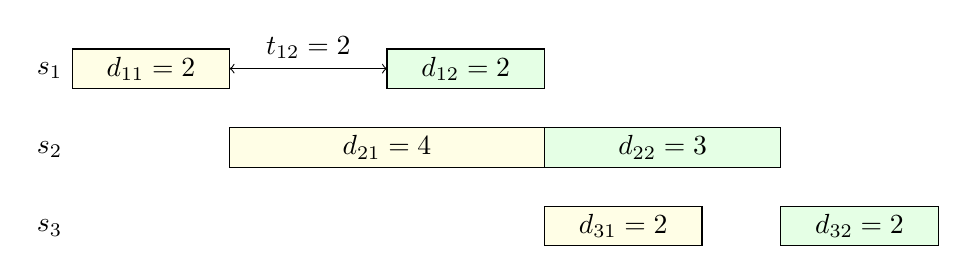
\begin{tikzpicture}

\draw[draw=black,fill=yellow!10] (0,3) rectangle node {$d_{11}=2$} (2,3.5);
\draw[draw=black,fill=yellow!10] (2,2) rectangle node {$d_{21}=4$} (6,2.5);
\draw[draw=black,fill=yellow!10] (6,1) rectangle node {$d_{31}=2$} (8,1.5);

\draw[draw=black,fill=green!10] (4,3) rectangle node {$d_{12}=2$} (6,3.5);
\draw[draw=black,fill=green!10] (6,2) rectangle node {$d_{22}=3$} (9,2.5);
\draw[draw=black,fill=green!10] (9,1) rectangle node {$d_{32}=2$} (11,1.5);

\node[above left] at (0,3) {$s_{1}$};
\node[above left] at (0,2) {$s_{2}$};
\node[above left] at (0,1) {$s_{3}$};

\draw[<->] (2,3.25) -- node[above] {$t_{12}=2$}(4,3.25);
\end{tikzpicture}
\end{figure}

We therefore have to wait for at least some time $t_{j_{1}j_{2}}$ between the end of the first task and the start of the second task in stage 1. The minimal time can be defined as

\begin{equation}
t_{j_{1}j_{2}} = \max(0,\max_{2 \leq i \leq s} \sum_{2\leq k \leq i} d_{kj_{1}} - \sum_{1 \leq k < i} d_{kj_{2}})
\end{equation}

In our example, the first term ($i=2$) is $4-2 = 2$, the second term ($i=3$) is $(4+2) - (2+3) = 1$, the required distance is therefore $t_{j_{1}j_{2}} = 2$. 

We can now consider a directed graph consisting of all jobs as nodes, plus one auxiliary node for both start and end, and links between all pairs $<i,j>$ of jobs 
with weight $d_{1i}+t_{ij}$, links between the auxiliary node and each job with weight zero, and links between each job $j$ and the auxiliary node with 
weight $\sum_{1 \leq i \leq s} d_{ij}$, i.e. the total duration of the job. We consider the minimal cost solution $C_{\textrm{TSP}}$ of the traveling salesman problem (TSP) on the resulting graph.

\begin{theorem}
\[
C_{\max} = C_{\textrm{TSP}} 
\]
\end{theorem}

Consider the sequence of jobs traversed by the optimal solution of the TSP, we name it $[j_{1}, j_{2},...,j_{n-1},j_{n}]$. If we schedule these jobs in order, 
starting at time zero, and leaving the required distance $t_{ij}$ between consecutive jobs, then the resulting schedule is a feasible schedule, 
shown in Figure~\ref{fig:proof}. The tasks of each job are scheduled without wait, two consecutive jobs never overlap for any stage, as the selected distances 
$t_{ij}$ on the tasks of the first stage ensure this. The length of the schedule is 
\begin{equation}
C_{\max} = \sum_{1 \leq k < n} d_{1k} + \sum_{1 \leq k < n} t_{k,k+1} + \sum_{1 \leq k \leq s} d_{kn}
\end{equation}
which is also the cost of the TSP solution used. The jobs in that sequence cannot be scheduled any tighter, if the distance between two consecutive jobs is less than $t_{ij}$, 
then the jobs will overlap in at least one stage.

Why is this solution an optimal solution to the scheduling problem? Suppose there exists another feasible schedule with a lower cost $C^{'}<C_{\textrm{TSP}}$. 
As the job order must be the same in each stage, that solution can also be represented by a job sequence. From that sequence we can construct 
another circuit in the graph which has the same cost $C^{'}$, which contradicts the assumption that the solution with $C_{\textrm{TSP}}$ is optimal.


\begin{figure}[htbp]
\caption{\label{fig:proof}Sketch of Proof (Stage View, Tasks colored by Job)}
\scalebox{0.6}{
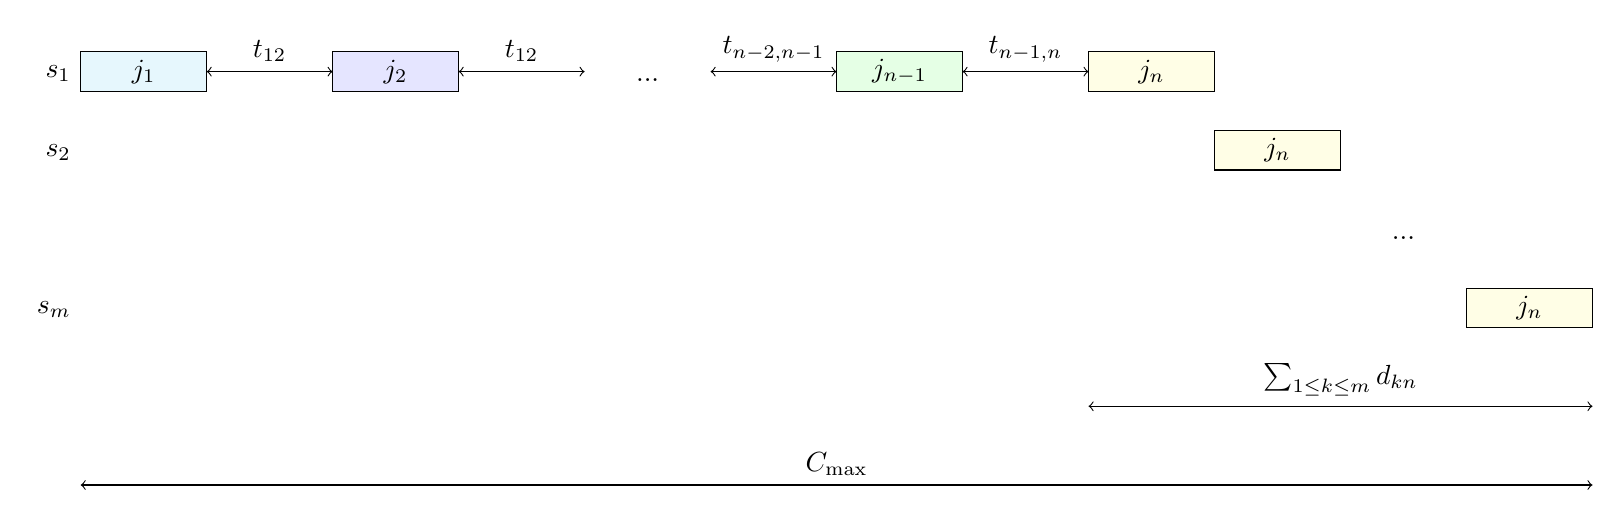
\begin{tikzpicture}[xscale=0.8]
\node[above left] at (0,3) {$s_{1}$};

\draw[draw=black,fill=cyan!10] (0,3) rectangle node {$j_{1}$} (2,3.5);
\draw[<->] (2,3.25) -- node[above] {$t_{12}$} (4,3.25);

\draw[draw=black,fill=blue!10] (4,3) rectangle node {$j_{2}$} (6,3.5);
\draw[<->] (6,3.25) -- node[above] {$t_{12}$} (8,3.25);
\node[above] at (9,3) {...};
\draw[<->] (10,3.25) -- node[above] {$t_{n-2,n-1}$} (12,3.25);
\draw[draw=black,fill=green!10] (12,3) rectangle node {$j_{n-1}$} (14,3.5);
\draw[<->] (14,3.25) -- node[above] {$t_{n-1,n}$} (16,3.25);
\draw[draw=black,fill=yellow!10] (16,3) rectangle node {$j_{n}$} (18,3.5);

\node[above left] at (0,2) {$s_{2}$};
\draw[draw=black,fill=yellow!10] (18,2) rectangle node {$j_{n}$} (20,2.5);
\node[above] at (21,1) {...};

\node[above left] at (0,0) {$s_{m}$};
\draw[draw=black,fill=yellow!10] (22,0) rectangle node {$j_{n}$} (24,0.5);

\draw[<->] (16,-1) -- node[above]{$\sum_{1 \leq k \leq m} d_{kn}$} (24,-1);
\draw[<->] (0,-2) -- node[above]{$C_{\max}$} (24,-2);

\end{tikzpicture}
}
\end{figure}

For this noWait flow-shop variant we can therefore generate optimal solutions by solving TSP problems, either with a generic solver or a specialized TSP solver like Concorde (\url{https://www.math.uwaterloo.ca/tsp/index.html}). 

\subsection{Use as Lower and Upper Bound?}
We may be able to use the cost of the no-wait flow-shop to create a lower bound on the no-wait hybrid flow-shop problem with multiple, identical machines. If every stage has $p$ identical machines, we would expect that there is not solution better than $C_{\textrm{TSP}}/p$.

We can partition the problem into $p$ independent sub-problems by partitioning the jobs into $p$ groups, and then solve each sub-problem to optimality. This would create an upper bound on the overall problem. We can also create a problem with $p$ auxiliary nodes and find $p$ cycles in the graph, forcing exactly one auxiliary node in each cycle. This would handle the best allocation of jobs to groups within the optimization routine. This probably cannot be expressed directly in Concorde, but would be possible using the cycle constraint in CHIP.




 

 




\end{document}
